\documentclass{ximera}

\input{../../../preamble.tex}


\definecolor{fvdnavy}{HTML}{071D43}
\definecolor{fvdcyan}{HTML}{20BFC6}
\definecolor{fvdcyanlight}{HTML}{EFFCFB}
\definecolor{fvdmagenta}{HTML}{F10D69}
\definecolor{fvdmagentalight}{HTML}{FFF1F7}
\definecolor{fvdtext}{HTML}{163044}





%=================================================
% Pedagogische omgevingen
% PDF: tcolorbox
% HTML: learning-box
%=================================================

\newenvironment{voorkennis}
{%
    \ifdefined\HCode
        \HCode{%
<section class="learning-box learning-box--prior">
<div class="learning-box__header">
<span class="learning-box__icon" aria-hidden="true"></span>
<span class="learning-box__title">Voorkennis</span>
</div>
<div class="learning-box__content">
        }%
        \begin{itemize}
    \else
       \begin{tcolorbox}[
    enhanced,
    breakable,
    colback=fvdcyanlight,
    colframe=fvdcyan,
    coltext=fvdtext,
    boxrule=0.5pt,
    leftrule=4pt,
    arc=4mm,
    outer arc=4mm,
    left=7mm,
    right=6mm,
    top=5mm,
    bottom=5mm,
    before skip=6mm,
    after skip=6mm,
    title=Voorkennis,
    coltitle=fvdcyan,
    fonttitle=\bfseries\Large,
    attach title to upper={\par\smallskip},
    boxed title style={
        empty,
        left=0mm,
        right=0mm,
        top=0mm,
        bottom=0mm
    },
    overlay={
        \draw[
            fvdcyan,
            line width=0.5pt
        ]
        ([xshift=42mm,yshift=-13mm]frame.north west)
        --
        ([xshift=-7mm,yshift=-13mm]frame.north east);
    }
]
        \begin{itemize}
    \fi
}
{%
    \end{itemize}
    \ifdefined\HCode
        \HCode{%
</div>
</section>
        }%
    \else
        \end{tcolorbox}
    \fi
}


\newenvironment{leerdoelen}
{%
    \ifdefined\HCode
        \HCode{%
<section class="learning-box learning-box--goals">
<div class="learning-box__header">
<span class="learning-box__icon" aria-hidden="true"></span>
<span class="learning-box__title">Leerdoelen</span>
</div>
<div class="learning-box__content">
        }%
        \begin{itemize}
    \else
\begin{tcolorbox}[
    enhanced,
    breakable,
    colback=fvdmagentalight,
    colframe=fvdmagenta,
    coltext=fvdtext,
    boxrule=0.5pt,
    leftrule=4pt,
    arc=4mm,
    outer arc=4mm,
    left=7mm,
    right=6mm,
    top=5mm,
    bottom=5mm,
    before skip=6mm,
    after skip=6mm,
    title=Leerdoelen,
    coltitle=fvdmagenta,
    fonttitle=\bfseries\Large,
    attach title to upper={\par\smallskip},
    boxed title style={
        empty,
        left=0mm,
        right=0mm,
        top=0mm,
        bottom=0mm
    },
    overlay={
        \draw[
            fvdmagenta,
            line width=0.5pt
        ]
        ([xshift=42mm,yshift=-13mm]frame.north west)
        --
        ([xshift=-7mm,yshift=-13mm]frame.north east);
    }
]
        \begin{itemize}
    \fi
}
{%
    \end{itemize}
    \ifdefined\HCode
        \HCode{%
</div>
</section>
        }%
    \else
        \end{tcolorbox}
    \fi
}



\title{Van kleine bijdragen naar integraal}
\author{Ingmar Herreman}

\begin{document}

% FVD_CHAPTER_DATA_START
% Automatisch gegenereerd uit index.tex.
% Niet handmatig aanpassen.
\fvdchapterdata{2}{Van oppervlakte naar integraal}{2}
% FVD_CHAPTER_DATA_END

% ============================================================
% ABSTRACT
% ============================================================

\begin{abstract}
In het vorige hoofdstuk konden we oppervlakten exact berekenen zolang
het gebied kon worden opgebouwd uit rechthoeken, driehoeken of
trapezia. Bij een gekromde grafiek werkt dat niet meer.

In dit hoofdstuk vertrekken we van één concreet oppervlakteprobleem.
We benaderen het gebied eerst met rechthoeken die te klein of te groot
zijn. Daarna maken we de verdeling steeds fijner. Zo groeit stap voor
stap het algemene idee van een Riemannsom en uiteindelijk van de
\textbf{bepaalde integraal}.

De centrale gedachte is:

\[
\boxed{
\text{oppervlakte}
\longrightarrow
\text{som van rechthoeken}
\longrightarrow
\text{steeds fijnere som}
\longrightarrow
\text{integraal}
}
\]
\end{abstract}

\maketitle

% ============================================================
% VOORKENNIS EN LEERDOELEN
% ============================================================

\begin{voorkennis}
    \item Je kan gewone en georiënteerde oppervlakte onderscheiden.
    \item Je kan positieve en negatieve bijdragen onder een grafiek interpreteren.
    \item Je kan een interval opdelen in deelintervallen.
    \item Je kan werken met somnotatie.
    \item Je kent het begrip limiet.
\end{voorkennis}

\begin{leerdoelen}
    \item Je kan een oppervlakte onder een kromme benaderen met rechthoeken.
    \item Je kan onder- en bovensommen interpreteren en vergelijken.
    \item Je kan uitleggen wat er gebeurt wanneer een verdeling steeds fijner wordt.
    \item Je kan een Riemannsom opstellen en de factoren in
          \(f(x_i^\ast)\Delta x_i\) interpreteren.
    \item Je kan het verschil uitleggen tussen linker- en rechtersommen
          enerzijds en onder- en bovensommen anderzijds.
    \item Je kan de bepaalde integraal interpreteren als de limiet van Riemannsommen.
    \item Je kent de betekenis van de notatie
          \(\displaystyle\int_a^b f(x)\,dx\).
    \item Je kan een bepaalde integraal interpreteren als georiënteerde oppervlakte.
    \item Je kan een gegeven Riemannsom analyseren en herkennen als een bepaalde integraal.
\end{leerdoelen}


% ============================================================
% 1. EEN CONCREET OPPERVLAKTEPROBLEEM
% ============================================================

\FVDsection{Hoe bepaal je de oppervlakte onder een kromme?}

Beschouw de functie

\[
f(x)=x^2
\]

op het interval \([0,4]\).

We willen de oppervlakte bepalen van het gebied tussen de grafiek van
\(f\), de \(x\)-as en de verticale rechte \(x=4\).

\begin{center}
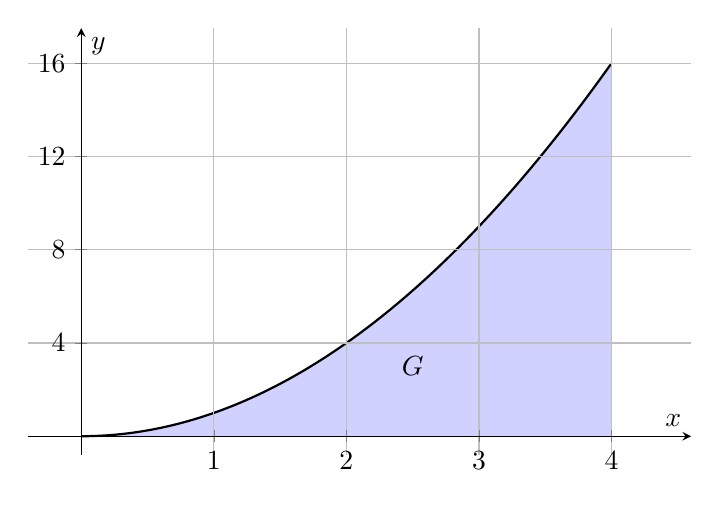
\begin{tikzpicture}
\begin{axis}[
    axis lines=middle,
    axis on top,
    xmin=-0.4, xmax=4.6,
    ymin=-0.8, ymax=17.5,
    xlabel={$x$},
    ylabel={$y$},
    xtick={0,1,2,3,4},
    ytick={0,4,8,12,16},
    grid=both,
    width=10cm,
    height=7cm
]
    \addplot[
        draw=none,
        fill=blue!18,
        domain=0:4,
        samples=120
    ] {x^2} \closedcycle;

    \addplot[
        black,
        thick,
        domain=0:4,
        samples=120
    ] {x^2};

    \draw[dashed] (axis cs:4,0)--(axis cs:4,16);
    \node at (axis cs:2.5,3) {$G$};
\end{axis}
\end{tikzpicture}
\end{center}

Het gebied \(G\) is geen rechthoek, driehoek of trapezium. De bovengrens
is immers gekromd.

Een rechtstreekse oppervlakteformule hebben we dus niet.

We kunnen de oppervlakte wel \textbf{inschatten}. Daarvoor vervangen we
het gekromde gebied tijdelijk door rechthoeken.

\[
\boxed{
\text{gekromd gebied}
\quad\longrightarrow\quad
\text{rechthoeken}
\quad\longrightarrow\quad
\text{som van oppervlakten}
}
\]


% ============================================================
% 2. ONDERSCHATTEN EN OVERSCHATTEN
% ============================================================

\FVDsection{Onderschattingen en overschattingen}

We verdelen \([0,4]\) eerst in vier gelijke deelintervallen:

\[
[0,1],\qquad [1,2],\qquad [2,3],\qquad [3,4].
\]

Elke rechthoek heeft dus breedte

\[
\Delta x=1.
\]

Omdat \(f(x)=x^2\) stijgt op \([0,4]\), kunnen we op elk deelinterval
twee natuurlijke rechthoeken tekenen.

\subsection*{Een onderschatting}

We nemen telkens de functiewaarde aan het \textbf{linker eindpunt} als
hoogte.

\begin{center}
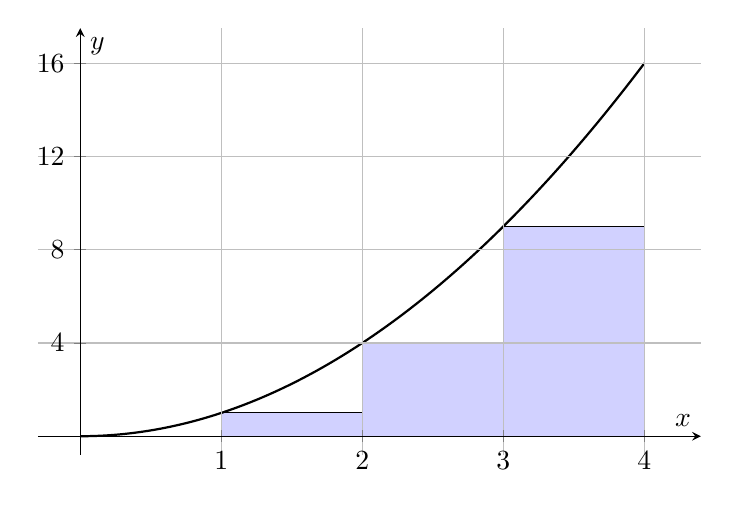
\begin{tikzpicture}
\begin{axis}[
    axis lines=middle,
    axis on top,
    xmin=-0.3, xmax=4.4,
    ymin=-0.8, ymax=17.5,
    xlabel={$x$},
    ylabel={$y$},
    xtick={0,1,2,3,4},
    ytick={0,4,8,12,16},
    grid=both,
    width=10cm,
    height=7cm
]
    \draw[fill=blue!18] (axis cs:0,0) rectangle (axis cs:1,0);
    \draw[fill=blue!18] (axis cs:1,0) rectangle (axis cs:2,1);
    \draw[fill=blue!18] (axis cs:2,0) rectangle (axis cs:3,4);
    \draw[fill=blue!18] (axis cs:3,0) rectangle (axis cs:4,9);

    \addplot[black,thick,domain=0:4,samples=120] {x^2};
\end{axis}
\end{tikzpicture}
\end{center}

De som van de rechthoeksoppervlakten is

\[
s_4
=
0^2\cdot1
+
1^2\cdot1
+
2^2\cdot1
+
3^2\cdot1.
\]

Dus

\[
s_4=0+1+4+9=14.
\]

De rechthoeken liggen volledig onder de grafiek. Daarom is

\[
\boxed{s_4<\text{exacte oppervlakte}}.
\]

We noemen \(s_4\) hier een \textbf{ondersom}.

\subsection*{Een overschatting}

We kunnen ook telkens de functiewaarde aan het \textbf{rechter eindpunt}
als hoogte nemen.

\begin{center}
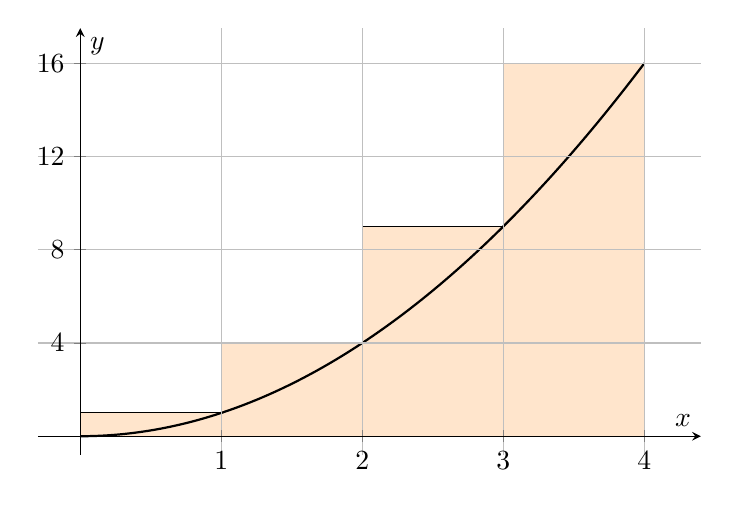
\begin{tikzpicture}
\begin{axis}[
    axis lines=middle,
    axis on top,
    xmin=-0.3, xmax=4.4,
    ymin=-0.8, ymax=17.5,
    xlabel={$x$},
    ylabel={$y$},
    xtick={0,1,2,3,4},
    ytick={0,4,8,12,16},
    grid=both,
    width=10cm,
    height=7cm
]
    \draw[fill=orange!20] (axis cs:0,0) rectangle (axis cs:1,1);
    \draw[fill=orange!20] (axis cs:1,0) rectangle (axis cs:2,4);
    \draw[fill=orange!20] (axis cs:2,0) rectangle (axis cs:3,9);
    \draw[fill=orange!20] (axis cs:3,0) rectangle (axis cs:4,16);

    \addplot[black,thick,domain=0:4,samples=120] {x^2};
\end{axis}
\end{tikzpicture}
\end{center}

Nu krijgen we

\[
S_4
=
1^2\cdot1
+
2^2\cdot1
+
3^2\cdot1
+
4^2\cdot1.
\]

Dus

\[
S_4=1+4+9+16=30.
\]

Deze rechthoeken liggen boven het gekromde gebied. Daarom

\[
\boxed{\text{exacte oppervlakte}<S_4}.
\]

We noemen \(S_4\) hier een \textbf{bovensom}.

Samen krijgen we onmiddellijk

\[
\boxed{
14<\text{exacte oppervlakte}<30
}.
\]

Dat is nog geen goede benadering, maar we hebben wel een belangrijk
idee gevonden: we kunnen de onbekende oppervlakte \textbf{insluiten}
tussen een onderschatting en een overschatting.


% ============================================================
% 3. STEEDS FIJNER VERDELEN
% ============================================================

\FVDsection{Wat gebeurt er als we fijner verdelen?}

Vier rechthoeken volgen de kromme nog erg grof. We kunnen daarom het
interval in meer, smallere stukken verdelen.

Voor \(n\) gelijke deelintervallen is de breedte

\[
\boxed{
\Delta x=\frac{4}{n}
}.
\]

Bij een stijgende functie zoals \(f(x)=x^2\) wordt de ondersom groter
wanneer de verdeling fijner wordt, terwijl de bovensom kleiner wordt.

\begin{center}
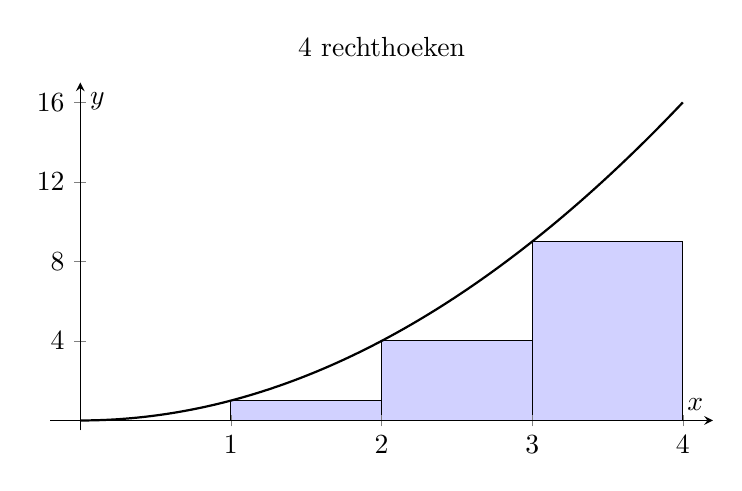
\begin{tikzpicture}
\begin{axis}[
    axis lines=middle,
    axis on top,
    xmin=-0.2, xmax=4.2,
    ymin=-0.5, ymax=17,
    xlabel={$x$},
    ylabel={$y$},
    xtick={0,1,2,3,4},
    ytick={0,4,8,12,16},
    width=10cm,
    height=6cm,
    title={4 rechthoeken}
]
    \draw[fill=blue!18] (axis cs:0,0) rectangle (axis cs:1,0);
    \draw[fill=blue!18] (axis cs:1,0) rectangle (axis cs:2,1);
    \draw[fill=blue!18] (axis cs:2,0) rectangle (axis cs:3,4);
    \draw[fill=blue!18] (axis cs:3,0) rectangle (axis cs:4,9);

    \addplot[black,thick,domain=0:4,samples=120] {x^2};
\end{axis}
\end{tikzpicture}

\vspace{0.8em}

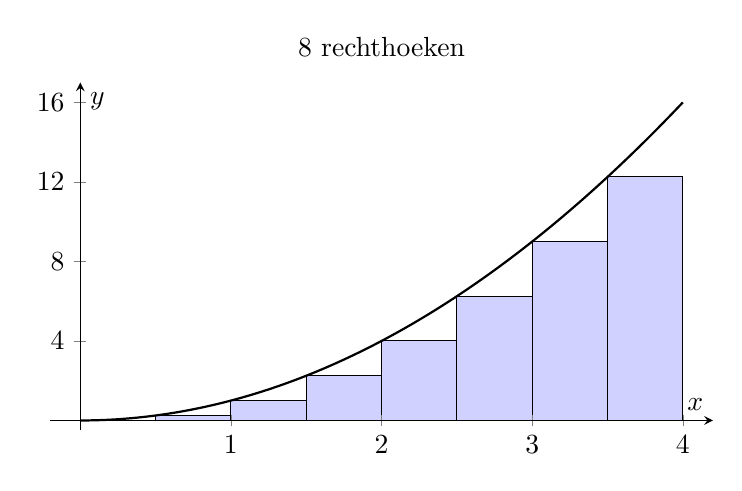
\begin{tikzpicture}
\begin{axis}[
    axis lines=middle,
    axis on top,
    xmin=-0.2, xmax=4.2,
    ymin=-0.5, ymax=17,
    xlabel={$x$},
    ylabel={$y$},
    xtick={0,1,2,3,4},
    ytick={0,4,8,12,16},
    width=10cm,
    height=6cm,
    title={8 rechthoeken}
]
    \draw[fill=blue!18] (axis cs:0,0) rectangle (axis cs:0.5,0);
    \draw[fill=blue!18] (axis cs:0.5,0) rectangle (axis cs:1,0.25);
    \draw[fill=blue!18] (axis cs:1,0) rectangle (axis cs:1.5,1);
    \draw[fill=blue!18] (axis cs:1.5,0) rectangle (axis cs:2,2.25);
    \draw[fill=blue!18] (axis cs:2,0) rectangle (axis cs:2.5,4);
    \draw[fill=blue!18] (axis cs:2.5,0) rectangle (axis cs:3,6.25);
    \draw[fill=blue!18] (axis cs:3,0) rectangle (axis cs:3.5,9);
    \draw[fill=blue!18] (axis cs:3.5,0) rectangle (axis cs:4,12.25);

    \addplot[black,thick,domain=0:4,samples=120] {x^2};
\end{axis}
\end{tikzpicture}
\end{center}

Visueel zien we wat er gebeurt: de lege ruimte tussen de rechthoeken en
de grafiek wordt kleiner.

Als we nog verder verfijnen, verwachten we

\[
s_4<s_8<s_{16}<\cdots<\text{exacte oppervlakte}
\]

en

\[
S_4>S_8>S_{16}>\cdots>\text{exacte oppervlakte}.
\]

Schematisch:

\[
\boxed{
\text{ondersommen}
\nearrow
\text{exacte waarde}
\qquad\text{en}\qquad
\text{bovensommen}
\searrow
\text{exacte waarde}
}
\]

De exacte oppervlakte verschijnt dus als een \textbf{grenswaarde} van
steeds fijnere sommen.

\begin{opmerking}
Het gebruik van onder- en bovensommen helpt ons vooral om het
limietidee zichtbaar te maken. Straks formuleren we het algemener:
de hoogte van een rechthoek hoeft niet noodzakelijk aan een linker- of
rechter eindpunt gekozen te worden.
\end{opmerking}


% ============================================================
% 4. VAN RECHTHOEKEN NAAR RIEMANNSOMMEN
% ============================================================

\FVDsection{Van rechthoeken naar een Riemannsom}

We maken het idee nu algemeen.

Verdeel een interval \([a,b]\) in deelintervallen:

\[
a=x_0<x_1<x_2<\cdots<x_n=b.
\]

Het \(i\)-de deelinterval is

\[
[x_{i-1},x_i]
\]

en heeft breedte

\[
\Delta x_i=x_i-x_{i-1}.
\]

In elk deelinterval kiezen we een punt

\[
x_i^\ast\in[x_{i-1},x_i].
\]

De functiewaarde

\[
f(x_i^\ast)
\]

gebruiken we als hoogte van een rechthoek.

De bijdrage van die rechthoek is dus

\[
f(x_i^\ast)\Delta x_i.
\]

Door alle bijdragen op te tellen, krijgen we

\[
\boxed{
\sum_{i=1}^{n} f(x_i^\ast)\Delta x_i
}.
\]

\begin{definitie}
Een som van de vorm

\[
\sum_{i=1}^{n} f(x_i^\ast)\Delta x_i
\]

noemen we een \textbf{Riemannsom} van \(f\) op \([a,b]\).
\end{definitie}

Elke term heeft een duidelijke betekenis:

\[
\underbrace{f(x_i^\ast)}_{\text{hoogte}}
\cdot
\underbrace{\Delta x_i}_{\text{breedte}}
=
\underbrace{f(x_i^\ast)\Delta x_i}_{\text{bijdrage}}.
\]

De volledige som stelt dus een benadering voor van de totale
georiënteerde bijdrage over het interval.


% ============================================================
% 5. LINKERSOM, RECHTERSOM, ONDERSOM EN BOVENSOM
% ============================================================

\FVDsection{Welke hoogte kiezen we?}

Er zijn verschillende manieren om de hoogte van de rechthoeken te kiezen.

\begin{itemize}
    \item Bij een \textbf{linkersom} nemen we in elk deelinterval het
          linker eindpunt.
    \item Bij een \textbf{rechtersom} nemen we in elk deelinterval het
          rechter eindpunt.
    \item Bij een \textbf{ondersom} kiezen we op elk deelinterval de
          kleinste functiewaarde.
    \item Bij een \textbf{bovensom} kiezen we op elk deelinterval de
          grootste functiewaarde.
\end{itemize}

Deze begrippen mogen we niet verwarren.

\begin{opmerking}
Bij een \textbf{stijgende} functie valt de linkersom samen met de
ondersom en de rechtersom met de bovensom.

Bij een \textbf{dalende} functie is het net omgekeerd.

Bij een functie die binnen een deelinterval eerst stijgt en daarna daalt,
hoeft geen van beide gelijk te zijn.
\end{opmerking}

Het onderscheid is dus:

\begin{center}
\textbf{Linkersom / rechtersom:} de plaats waar we de functie evalueren.

\textbf{Ondersom / bovensom:} de kleinste of grootste functiewaarde
op elk deelinterval.
\end{center}


% ============================================================
% 6. VAN STEEDS FIJNERE SOMMEN NAAR EEN INTEGRAAL
% ============================================================

\FVDsection{Van Riemannsommen naar de bepaalde integraal}

Een Riemannsom is nog maar een benadering.

We maken de verdeling daarom steeds fijner. De breedtes
\(\Delta x_i\) worden steeds kleiner en de rechthoeken kunnen de grafiek
steeds beter volgen.

Als de Riemannsommen daarbij naar éénzelfde getal naderen, onafhankelijk
van de precieze keuze van de punten \(x_i^\ast\), noemen we die
grenswaarde de \textbf{bepaalde integraal}.

\begin{definitie}
Voor een integreerbare functie \(f\) op \([a,b]\) is

\[
\boxed{
\int_a^b f(x)\,dx
=
\lim
\sum_{i=1}^{n}f(x_i^\ast)\Delta x_i
}
\]

waarbij de grootste breedte van de deelintervallen naar \(0\) gaat.
\end{definitie}

Voor \(n\) even brede deelintervallen geldt

\[
\Delta x=\frac{b-a}{n}.
\]

Dan schrijven we het idee vaak als

\[
\boxed{
\int_a^b f(x)\,dx
=
\lim_{n\to\infty}
\sum_{i=1}^{n}f(x_i^\ast)\Delta x
}.
\]

De integraal ontstaat dus niet uit het niets. Ze is de grenswaarde van
sommen van steeds kleinere bijdragen:

\[
\text{kleine bijdrage}
\;\longrightarrow\;
\text{som}
\;\longrightarrow\;
\text{steeds fijnere som}
\;\longrightarrow\;
\text{limiet}
\;\longrightarrow\;
\text{integraal}.
\]


% ============================================================
% 7. DE INTEGRAALNOTATIE
% ============================================================

\FVDsection{De integraalnotatie lezen}

In

\[
\int_a^b f(x)\,dx
\]

heeft elk symbool een betekenis.

\[
\underbrace{\int}_{\text{integraalteken}}
\quad
\underbrace{f(x)}_{\text{integrand}}
\quad
\underbrace{dx}_{\text{integratievariabele}}
\]

met \(a\) als \textbf{ondergrens} en \(b\) als \textbf{bovengrens}.

We lezen

\[
\int_a^b f(x)\,dx
\]

als:

\begin{center}
``de bepaalde integraal van \(f(x)\) van \(a\) tot \(b\)''.
\end{center}

Het integraalteken \(\int\) is historisch ontstaan uit een langgerekte
letter \(S\): het verwijst naar het optellen van vele kleine bijdragen.

Ook \(dx\) sluit aan bij de Riemannsom. Daar werkten we met kleine
breedtes \(\Delta x\). In de limiet worden deze breedtes willekeurig
klein.


% ============================================================
% 8. GEORIENTEERDE OPPERVLAKTE
% ============================================================

\FVDsection{Integraal en georiënteerde oppervlakte}

Tot nu toe lag onze eerste voorbeeldfunctie boven de \(x\)-as. Maar de
definitie met Riemannsommen werkt ook wanneer een grafiek onder de
\(x\)-as ligt.

Als

\[
f(x_i^\ast)<0,
\]

dan is

\[
f(x_i^\ast)\Delta x_i<0.
\]

Zo worden gebieden onder de \(x\)-as automatisch negatief meegeteld.

\begin{opmerking}
Voor een integreerbare functie \(f\) stelt

\[
\int_a^b f(x)\,dx
\]

de \textbf{georiënteerde oppervlakte} voor tussen de grafiek van \(f\),
de \(x\)-as en de verticale rechten \(x=a\) en \(x=b\).

Gebieden boven de \(x\)-as leveren positieve bijdragen en gebieden onder
de \(x\)-as negatieve bijdragen.
\end{opmerking}

\begin{center}
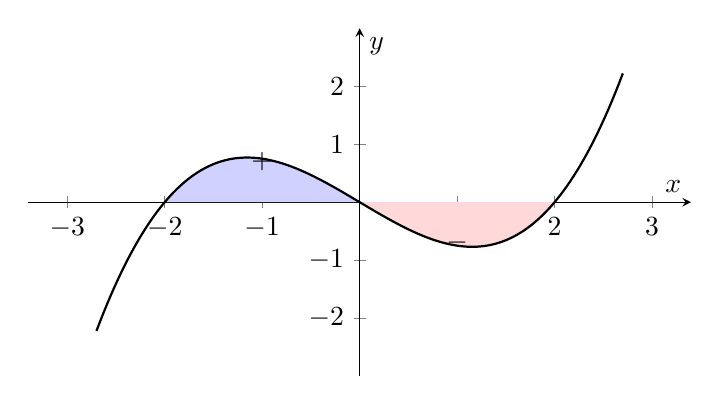
\begin{tikzpicture}
\begin{axis}[
    axis lines=middle,
    xmin=-3.4, xmax=3.4,
    ymin=-3, ymax=3,
    xlabel={$x$},
    ylabel={$y$},
    xtick={-3,-2,-1,0,1,2,3},
    ytick={-2,-1,0,1,2},
    width=10cm,
    height=6cm
]
    \addplot[
        draw=none,
        fill=blue!18,
        domain=-2:0,
        samples=80
    ] {0.25*x*(x+2)*(x-2)} \closedcycle;

    \addplot[
        draw=none,
        fill=red!15,
        domain=0:2,
        samples=80
    ] {0.25*x*(x+2)*(x-2)} \closedcycle;

    \addplot[
        black,
        thick,
        domain=-2.7:2.7,
        samples=150
    ] {0.25*x*(x+2)*(x-2)};

    \node at (axis cs:-1,0.7) {$+$};
    \node at (axis cs:1,-0.7) {$-$};
\end{axis}
\end{tikzpicture}
\end{center}

Daarom kan

\[
\int_a^b f(x)\,dx
\]

positief, nul of negatief zijn.

\begin{opmerking}
Een bepaalde integraal is niet automatisch de \textbf{gewone}
oppervlakte. Wanneer de grafiek onder de \(x\)-as ligt, moeten we voor
de gewone oppervlakte de absolute grootte van dat gebied nemen.
\end{opmerking}


% ============================================================
% 9. EEN KEER EXACT VIA EEN RIEMANNSOM
% ============================================================

\FVDsection{Eén keer exact rekenen met een Riemannsom}

We hebben gezien hoe Riemannsommen een oppervlakte benaderen. Nu willen
we één keer exact zien hoe zo'n som in de limiet een bepaalde integraal
wordt.

Beschouw

\[
f(x)=x^2
\]

op \([0,2]\).

We verdelen \([0,2]\) in \(n\) gelijke deelintervallen. Dan

\[
\Delta x=\frac{2}{n}.
\]

We kiezen telkens het rechter eindpunt:

\[
x_i=\frac{2i}{n}.
\]

De rechtersom is

\[
R_n
=
\sum_{i=1}^{n}
f\left(\frac{2i}{n}\right)\frac{2}{n}.
\]

Omdat \(f(x)=x^2\),

\[
R_n
=
\sum_{i=1}^{n}
\left(\frac{2i}{n}\right)^2\frac{2}{n}.
\]

Dus

\[
R_n
=
\sum_{i=1}^{n}
\frac{8i^2}{n^3}
=
\frac{8}{n^3}
\sum_{i=1}^{n}i^2.
\]

We gebruiken

\[
\sum_{i=1}^{n}i^2
=
\frac{n(n+1)(2n+1)}{6}.
\]

Daarom

\[
R_n
=
\frac{8}{n^3}
\cdot
\frac{n(n+1)(2n+1)}{6}
\]

en dus

\[
R_n
=
\frac{4(n+1)(2n+1)}{3n^2}.
\]

We laten nu \(n\) naar oneindig gaan:

\[
\int_0^2x^2\,dx
=
\lim_{n\to\infty}R_n
=
\lim_{n\to\infty}
\frac{4(n+1)(2n+1)}{3n^2}.
\]

Na delen door \(n^2\):

\[
\int_0^2x^2\,dx
=
\lim_{n\to\infty}
\frac{4\left(1+\frac1n\right)
\left(2+\frac1n\right)}{3}
=
\boxed{\frac83}.
\]

We hebben dus rechtstreeks vanuit de definitie gevonden:

\[
\boxed{
\int_0^2x^2\,dx=\frac83
}.
\]

\begin{opmerking}
De formule voor \(\sum i^2\) is hier alleen een hulpmiddel om één keer
exact te zien hoe een Riemannsom naar een integraal leidt.

Het is \textbf{niet} de bedoeling om voortaan elke integraal op deze
manier te berekenen. We zoeken juist een veel efficiëntere methode.
\end{opmerking}


% ============================================================
% 10. EEN RIEMANNSOM ANALYSEREN
% ============================================================

\FVDsection{Een som herkennen als integraal}

Een belangrijke vaardigheid is ook de omgekeerde beweging: vanuit een
gegeven som herkennen welke bepaalde integraal ze voorstelt.

Beschouw

\[
\lim_{n\to\infty}
\sum_{i=1}^{n}
\left(
1+\left(\frac{3i}{n}\right)^2
\right)
\frac{3}{n}.
\]

We vergelijken dit met

\[
\sum_{i=1}^{n}f(x_i^\ast)\Delta x.
\]

Eerst herkennen we de breedte:

\[
\Delta x=\frac{3}{n}.
\]

Omdat

\[
\Delta x=\frac{b-a}{n},
\]

heeft het interval lengte \(3\). De punten

\[
x_i=\frac{3i}{n}
\]

zijn de rechter eindpunten van een verdeling van \([0,3]\).

Vervolgens herkennen we

\[
f(x_i)
=
1+\left(\frac{3i}{n}\right)^2.
\]

Dus

\[
f(x)=1+x^2.
\]

Daarom stelt de limiet voor:

\[
\boxed{
\int_0^3(1+x^2)\,dx
}.
\]

\begin{opmerking}
Bij dit soort analysevragen zoeken we systematisch naar

\[
\boxed{
\text{interval}
\qquad
\text{breedte}
\qquad
\text{functiewaarde}
}
\]

of in symbolen:

\[
[a,b],
\qquad
\Delta x,
\qquad
f(x_i^\ast).
\]
\end{opmerking}


% ============================================================
% 11. VAN BEGRIJPEN NAAR BEREKENEN
% ============================================================

\FVDsection{Van begrijpen naar berekenen}

We hebben nu dezelfde wiskundige grootheid vanuit verschillende
gezichtspunten leren kennen:

\[
\text{som van kleine bijdragen}
\;\longrightarrow\;
\text{limiet}
\;\longleftrightarrow\;
\text{bepaalde integraal}
\;\longleftrightarrow\;
\text{georiënteerde oppervlakte}.
\]

Voor

\[
\int_0^2x^2\,dx
\]

hebben we zelfs via de definitie gevonden dat

\[
\int_0^2x^2\,dx=\frac83.
\]

Maar de berekening was omslachtig.

Als we voor elke nieuwe veeltermfunctie opnieuw een Riemannsom volledig
zouden moeten uitwerken, zou integraalrekening weinig praktisch zijn.

Er moet dus een snellere manier bestaan.

Uit de afgeleidenleer kennen we bijvoorbeeld

\[
\frac{d}{dx}\left(\frac{x^3}{3}\right)=x^2.
\]

Dat roept een nieuwe vraag op:

\[
\boxed{
\text{Kunnen we het afleiden omkeren om integralen sneller te berekenen?}
}
\]

Dat is precies de stap die we in het volgende hoofdstuk zetten.

\end{document}



